\section{Introduction}\label{sec:introduction}

The landscape of manufacturing and control systems has evolved dramatically in recent decades, with modern industrial environments demanding unprecedented levels of adaptability, modularity, and system integration. This evolution has given rise to sophisticated distributed control architectures, commonly referred to as Component-Based industrial Automation Systems (CBAS) or industrial Cyber-Physical Systems (iCPS), which represent a paradigm shift from traditional centralized control approaches. The IEC 61499 standard has emerged as a key enabler for engineering these complex systems, providing a vendor-independent, component-based model for distributed control applications.

However, the increased complexity and distributed nature of these systems pose significant verification and validation (V\&V) challenges. Traditional V\&V techniques, such as simulation and testing, are often inadequate for ensuring the high levels of dependability, safety, and reliability required, particularly in safety-critical domains like nuclear material handling or power grid protection. While simulation is invaluable for assessing general system behavior, it cannot explore the entire state space of complex industrial software, meaning it can show the presence of bugs but not their absence.

To address this gap, formal methods offer a mathematically rigorous approach to system verification. Model checking, in particular, is an automated technique that systematically explores all reachable states of a system model to verify whether it satisfies a given set of formal specifications, typically expressed in temporal logic. Despite its power to uncover subtle design flaws that simulation might miss, the adoption of model checking in industrial practice has been limited. This is often due to challenges such as the state-space explosion problem, the need for specialized expertise to create formal models, and a lack of user-friendly tools that integrate seamlessly into the existing engineering lifecycle.

This chapter presents an integrated, model-based framework designed to bridge this gap. It leverages the IEC 61499 standard not only for controller design but also for modeling the system's environment (the "plant"), creating a comprehensive closed-loop model suitable for rigorous verification. The framework incorporates a seamless toolchain that automates the translation of IEC 61499 designs into a formal representation for a powerful model checker, and provides intuitive tools for analyzing the results. Key contributions of this framework include a novel notation for introducing non-determinism into plant models to make verification more realistic and a specific methodology for verifying the correctness of runtime safety monitors.

The chapter is structured as follows. Section \ref{sec:iec61499} provides an overview of the IEC 61499 standard. Section \ref{sec:formal_verification} introduces the principles of formal verification and the closed-loop modeling paradigm. Section \ref{sec:toolchain} details the components of the integrated toolchain and the associated methodologies for enhancing verification. Section \ref{sec:case_studies} demonstrates the practical application of the framework through several case studies, from laboratory-scale systems to a safety-critical industrial machine. Finally, Section \ref{sec:conclusion_chapter2} concludes the chapter and discusses future research directions.

\section{The IEC 61499 Standard for Distributed Automation}\label{sec:iec61499}

The IEC 61499 standard provides a reference architecture for the development of distributed control systems. It was conceived as a successor to the prevalent IEC 61131-3 standard, moving beyond the limitations of centralized, PLC-centric logic to support the demands of modern, distributed iCPS.

At the core of the standard is the Function Block (FB), a reusable software component that encapsulates data and algorithms. FBs interact through a well-defined graphical interface consisting of event and data inputs and outputs. The execution of logic within an FB is event-driven; an input event triggers the execution of associated algorithms and may result in the emission of one or more output events, propagating the flow of control through the network.

The standard defines several types of FBs, with the most fundamental being the Basic Function Block (BFB). The internal logic of a BFB is defined by an Execution Control Chart (ECC), which is a state machine that dictates the sequence of algorithm execution in response to input events. A Composite Function Block (CFB), in contrast, contains an internal network of other interconnected FBs, enabling hierarchical system design. This component-based, event-driven nature makes IEC 61499 inherently suited for modeling modular, reconfigurable, and distributed systems.

Despite these advantages, the verification of IEC 61499 applications is a recognized challenge. The concurrent and distributed nature of the systems can lead to complex emergent behaviors that are difficult to predict. Furthermore, ambiguities in the standard's original execution semantics led to different interpretations by tool vendors, creating portability and interoperability issues that formal modeling can help to identify and resolve.

\section{Formal Verification for IEC 61499 Systems}\label{sec:formal_verification}

Formal verification is the process of using mathematical methods to prove or disprove the correctness of a system with respect to a set of formal specifications. Model checking is a prominent formal verification technique that automates this process. It operates on a finite-state model of the system, systematically exploring all possible execution paths to check if they satisfy properties expressed in a formal language, such as Linear Temporal Logic (LTL) or Computation Tree Logic (CTL). If a property is violated, the model checker produces a counterexample—a specific trace of execution that demonstrates the failure.

\subsection{The Closed-Loop Modeling Paradigm}

A crucial aspect of applying model checking effectively to control systems is the adoption of a closed-loop modeling approach. Verifying a controller in isolation (open-loop) requires making assumptions about all possible inputs it might receive from its environment, which often leads to an unmanageably large state space and can produce spurious counterexamples that are not possible in the real system.

A closed-loop model, by contrast, includes a formal model of the plant—the physical process or environment the controller interacts with. This model constrains the inputs to the controller to only those that are physically possible, drastically reducing the reachable state space and leading to more meaningful verification results. This architecture, encompassing both the controller and the plant, allows for the verification of system-level properties that involve interactions between the two.

Figure \ref{fig:closed_loop_example} illustrates this closed-loop concept using a practical example of two pneumatic cylinders. The figure shows how the control program (consisting of horizontal and vertical cylinder controllers) interacts with plant models that simulate the physical behavior of the cylinders. The HMI visualization on the right demonstrates the real-time state of the system, including the critical situation where both cylinders are extended simultaneously—a condition that should be avoided. This visual representation helps engineers understand how the closed-loop configuration enables comprehensive verification by modeling both the control logic and the physical system behavior.

\begin{figure}[h]
\centering
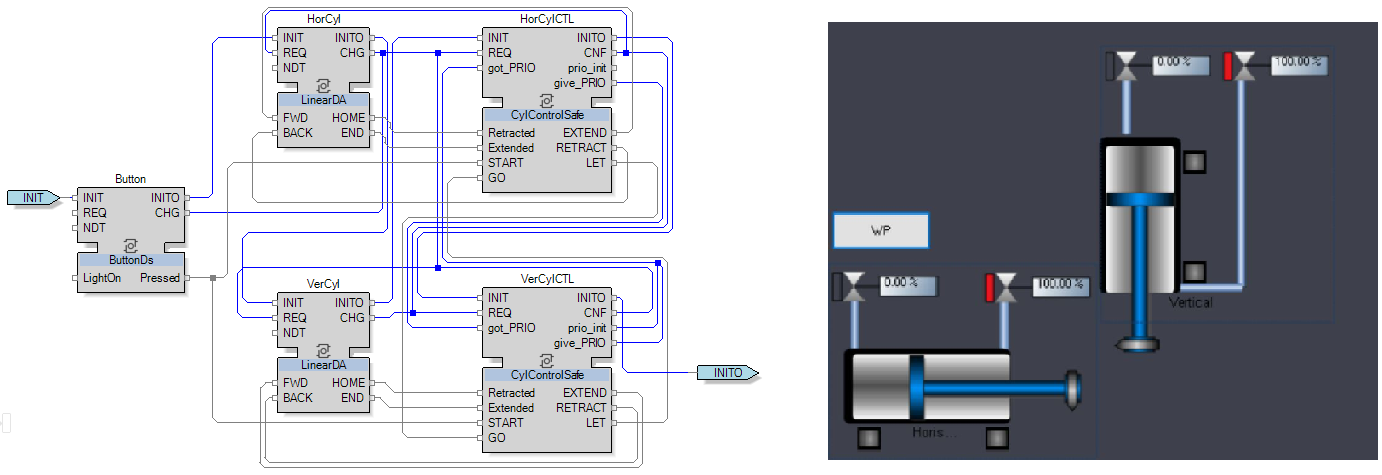
\includegraphics[width=0.8\textwidth]{chapters/images/chapter2/wholesystem_withhmi.png}
\caption{Example of a closed-loop system: two pneumatic orthogonal cylinders with their control program and HMI visualization. The system demonstrates how controllers and plant models interact in a closed-loop configuration for comprehensive verification.}
\label{fig:closed_loop_example}
\end{figure}

\subsection{From Simulation to Verification Models}

The IEC 61499 standard is well-suited for closed-loop modeling because the same component-based language can be used to model both the controller and the plant. This allows for a seamless transition from simulation to formal verification.

Initially, a detailed plant model, often equivalent to a hybrid automaton with continuous dynamics, can be created for simulation-in-the-loop to test the overall system behavior and provide visualization. For formal verification, this detailed model is then abstracted into a simpler, discrete-state model that captures the essential behaviors relevant to the properties being checked, but omits complexities like continuous dynamics that are computationally expensive for model checkers to handle. This dual-model approach allows engineers to use familiar tools for design and simulation, while enabling a pathway to rigorous formal verification.

\section{An Integrated Verification Toolchain and Methodology}\label{sec:toolchain}

To make formal verification practical for automation engineers, a seamless and highly automated toolchain is required. The framework presented here integrates industry-standard design environments with a powerful open-source model checker, facilitated by a custom model generator and advanced analysis tools.

\subsection{Overview of the Toolchain}

The proposed workflow connects the design, verification, and analysis phases into a cohesive process.

The toolchain consists of the following key components:

\begin{itemize}
\item \textbf{IEC 61499 Design Environment}: The process begins in an IEC 61499-compliant IDE, such as EcoStruxure™ Automation Expert or the open-source Function Blocks Modelling Environment (FBME) , where the controller and plant FBs are designed and simulated.

\item \textbf{Formal Model Generator (fb2smv)}: The fb2smv tool automatically translates the IEC 61499 application, described in its standard XML format, into a formal model in the SMV (Symbolic Model Verifier) language. This tool uses Abstract State Machines (ASM) as an intermediate model to handle the translation of the ECCs, algorithms, and network connections.

\item \textbf{Symbolic Model Checker (NuSMV)}: The generated SMV model is fed into NuSMV, an open-source symbolic model checker. NuSMV verifies the model against the specified LTL or CTL properties and, if a violation is found, generates a counterexample trace.

\item \textbf{Counterexample Analysis Environment (FBME)}: Analyzing the raw text output of a model checker can be difficult and unintuitive. Tools like FBME have been enhanced with trace visualization capabilities that import the counterexample from NuSMV and map it back onto the original graphical IEC 61499 model. This allows engineers to step through the failure trace visually, see the state of ECCs and variable values at each step, and use causal analysis to pinpoint the root cause of the error.
\end{itemize}

Figure \ref{fig:fbme_cex} demonstrates the FBME counterexample analysis interface, which provides a crucial bridge between formal verification results and practical debugging. The interface shows the execution trace in a visual format, allowing engineers to step through each state transition and observe how variables change over time. This visualization makes it possible to identify the exact sequence of events that led to a property violation, transforming abstract model checking results into actionable insights for system improvement.

\begin{figure}[h]
\centering
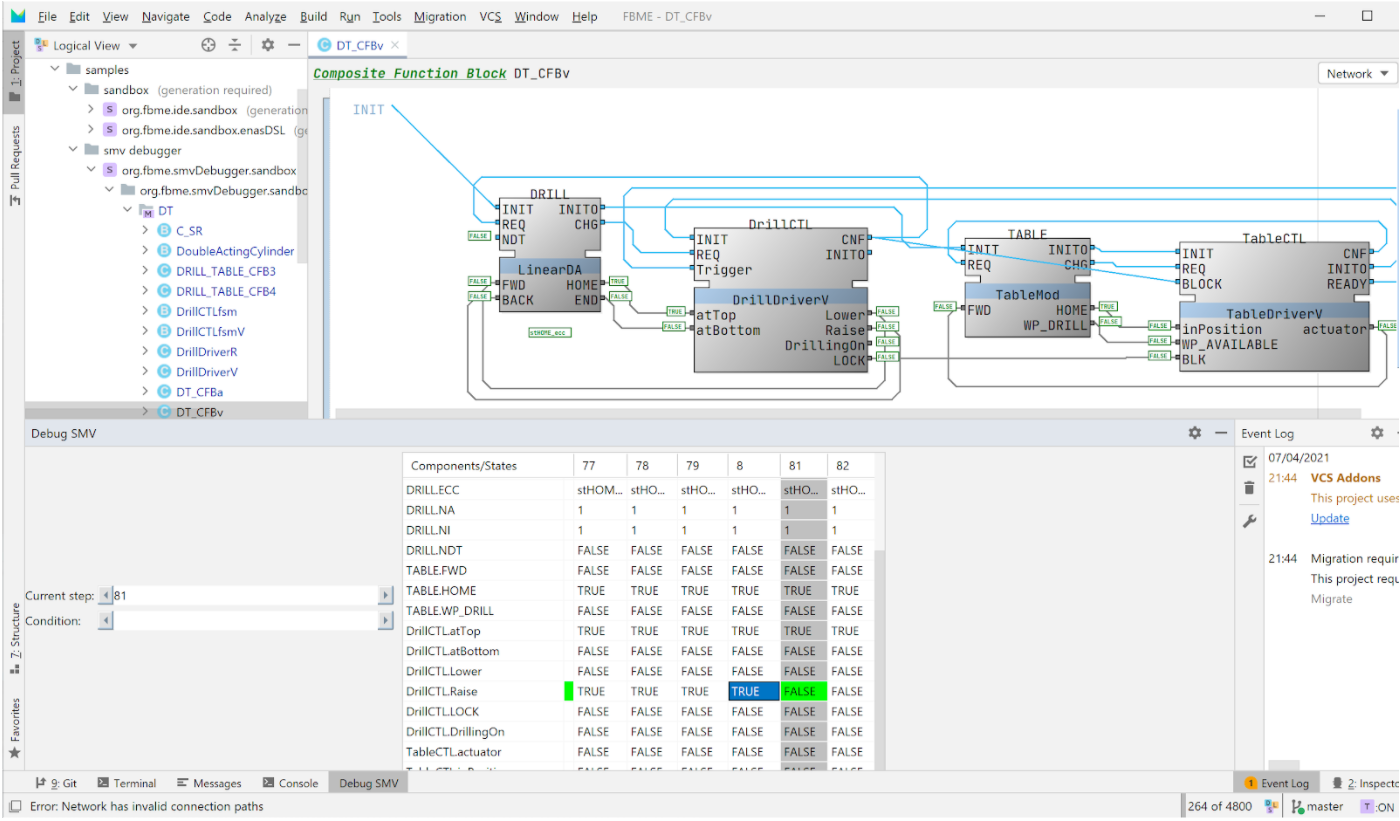
\includegraphics[width=0.7\textwidth]{chapters/images/chapter2/FBME_cex.png}
\caption{FBME counterexample analysis interface showing trace visualization and state analysis capabilities for debugging formal verification results.}
\label{fig:fbme_cex}
\end{figure}

\subsection{Enhancing Plant Models with Non-Deterministic Transitions (NDT)}

A key challenge in creating abstracted plant models for verification is ensuring they are realistic enough to capture potential failures. A purely deterministic model, where an action takes a fixed amount of time, may fail to uncover timing-related bugs, such as collisions that occur only when one axis moves faster or slower than another.

To address this, this framework introduces a problem-oriented notation for Non-Deterministic Transitions (NDT) directly within the ECC of an IEC 61499 plant model. An NDT represents a transition that can fire at an arbitrary time after it becomes enabled. For example, in a model of a linear axis, an NDT can be used to model the unknown duration of the motion between two points.

When the fb2smv tool encounters an NDT event, it translates it into a non-deterministic choice in the SMV model. This instructs the model checker to explore all possible timings for that transition, effectively simulating a wide range of real-world scenarios (e.g., different relative speeds between concurrent movements) and enabling the detection of subtle, timing-dependent design flaws that would be difficult to find through simulation alone. This ability to govern and selectively inject non-determinism is a powerful feature for performing targeted formal verification under specific stress conditions.

\subsection{A Methodology for Verifying Runtime Monitors}

In addition to offline verification at the design stage, many safety-critical systems utilize online verification through runtime monitors. These monitors, often implemented as FBs themselves, observe the system during operation and signal an error if a safety property is violated. However, a monitor only improves system safety if its own correctness is guaranteed.

Verifying a monitor presents a unique challenge. Traditional open-loop model checking, where the monitor's inputs are allowed to change arbitrarily, will often produce spurious counterexamples. This is because it allows input combinations that are semantically impossible in a real IEC 61499 system, such as data being transferred without a corresponding event firing.

To solve this, a methodology is proposed for the closed-loop model checking of monitors using a non-deterministic twin (ND twin) of the controller it supervises. The ND twin is a simplified FB that abstracts the controller's logic but is designed to produce every possible valid combination of its outputs. It achieves this by using NDTs to allow arbitrary transitions between its key states (e.g., EXTEND, RETRACT, STOP).

Figure \ref{fig:controller_ndts} illustrates the transformation from a timer-based controller to one using non-deterministic transitions for formal verification. The left side shows the original drill controller that uses external timer function blocks (E\_DELAY) to model time delays, which are computationally expensive for model checking. The right side shows the modified controller where these timer-based delays have been replaced with NDT events, significantly reducing the state space while maintaining the essential behavioral characteristics needed for verification. This transformation enables efficient formal verification while preserving the critical timing-dependent behaviors that could lead to safety violations.

\begin{figure}[h]
\centering
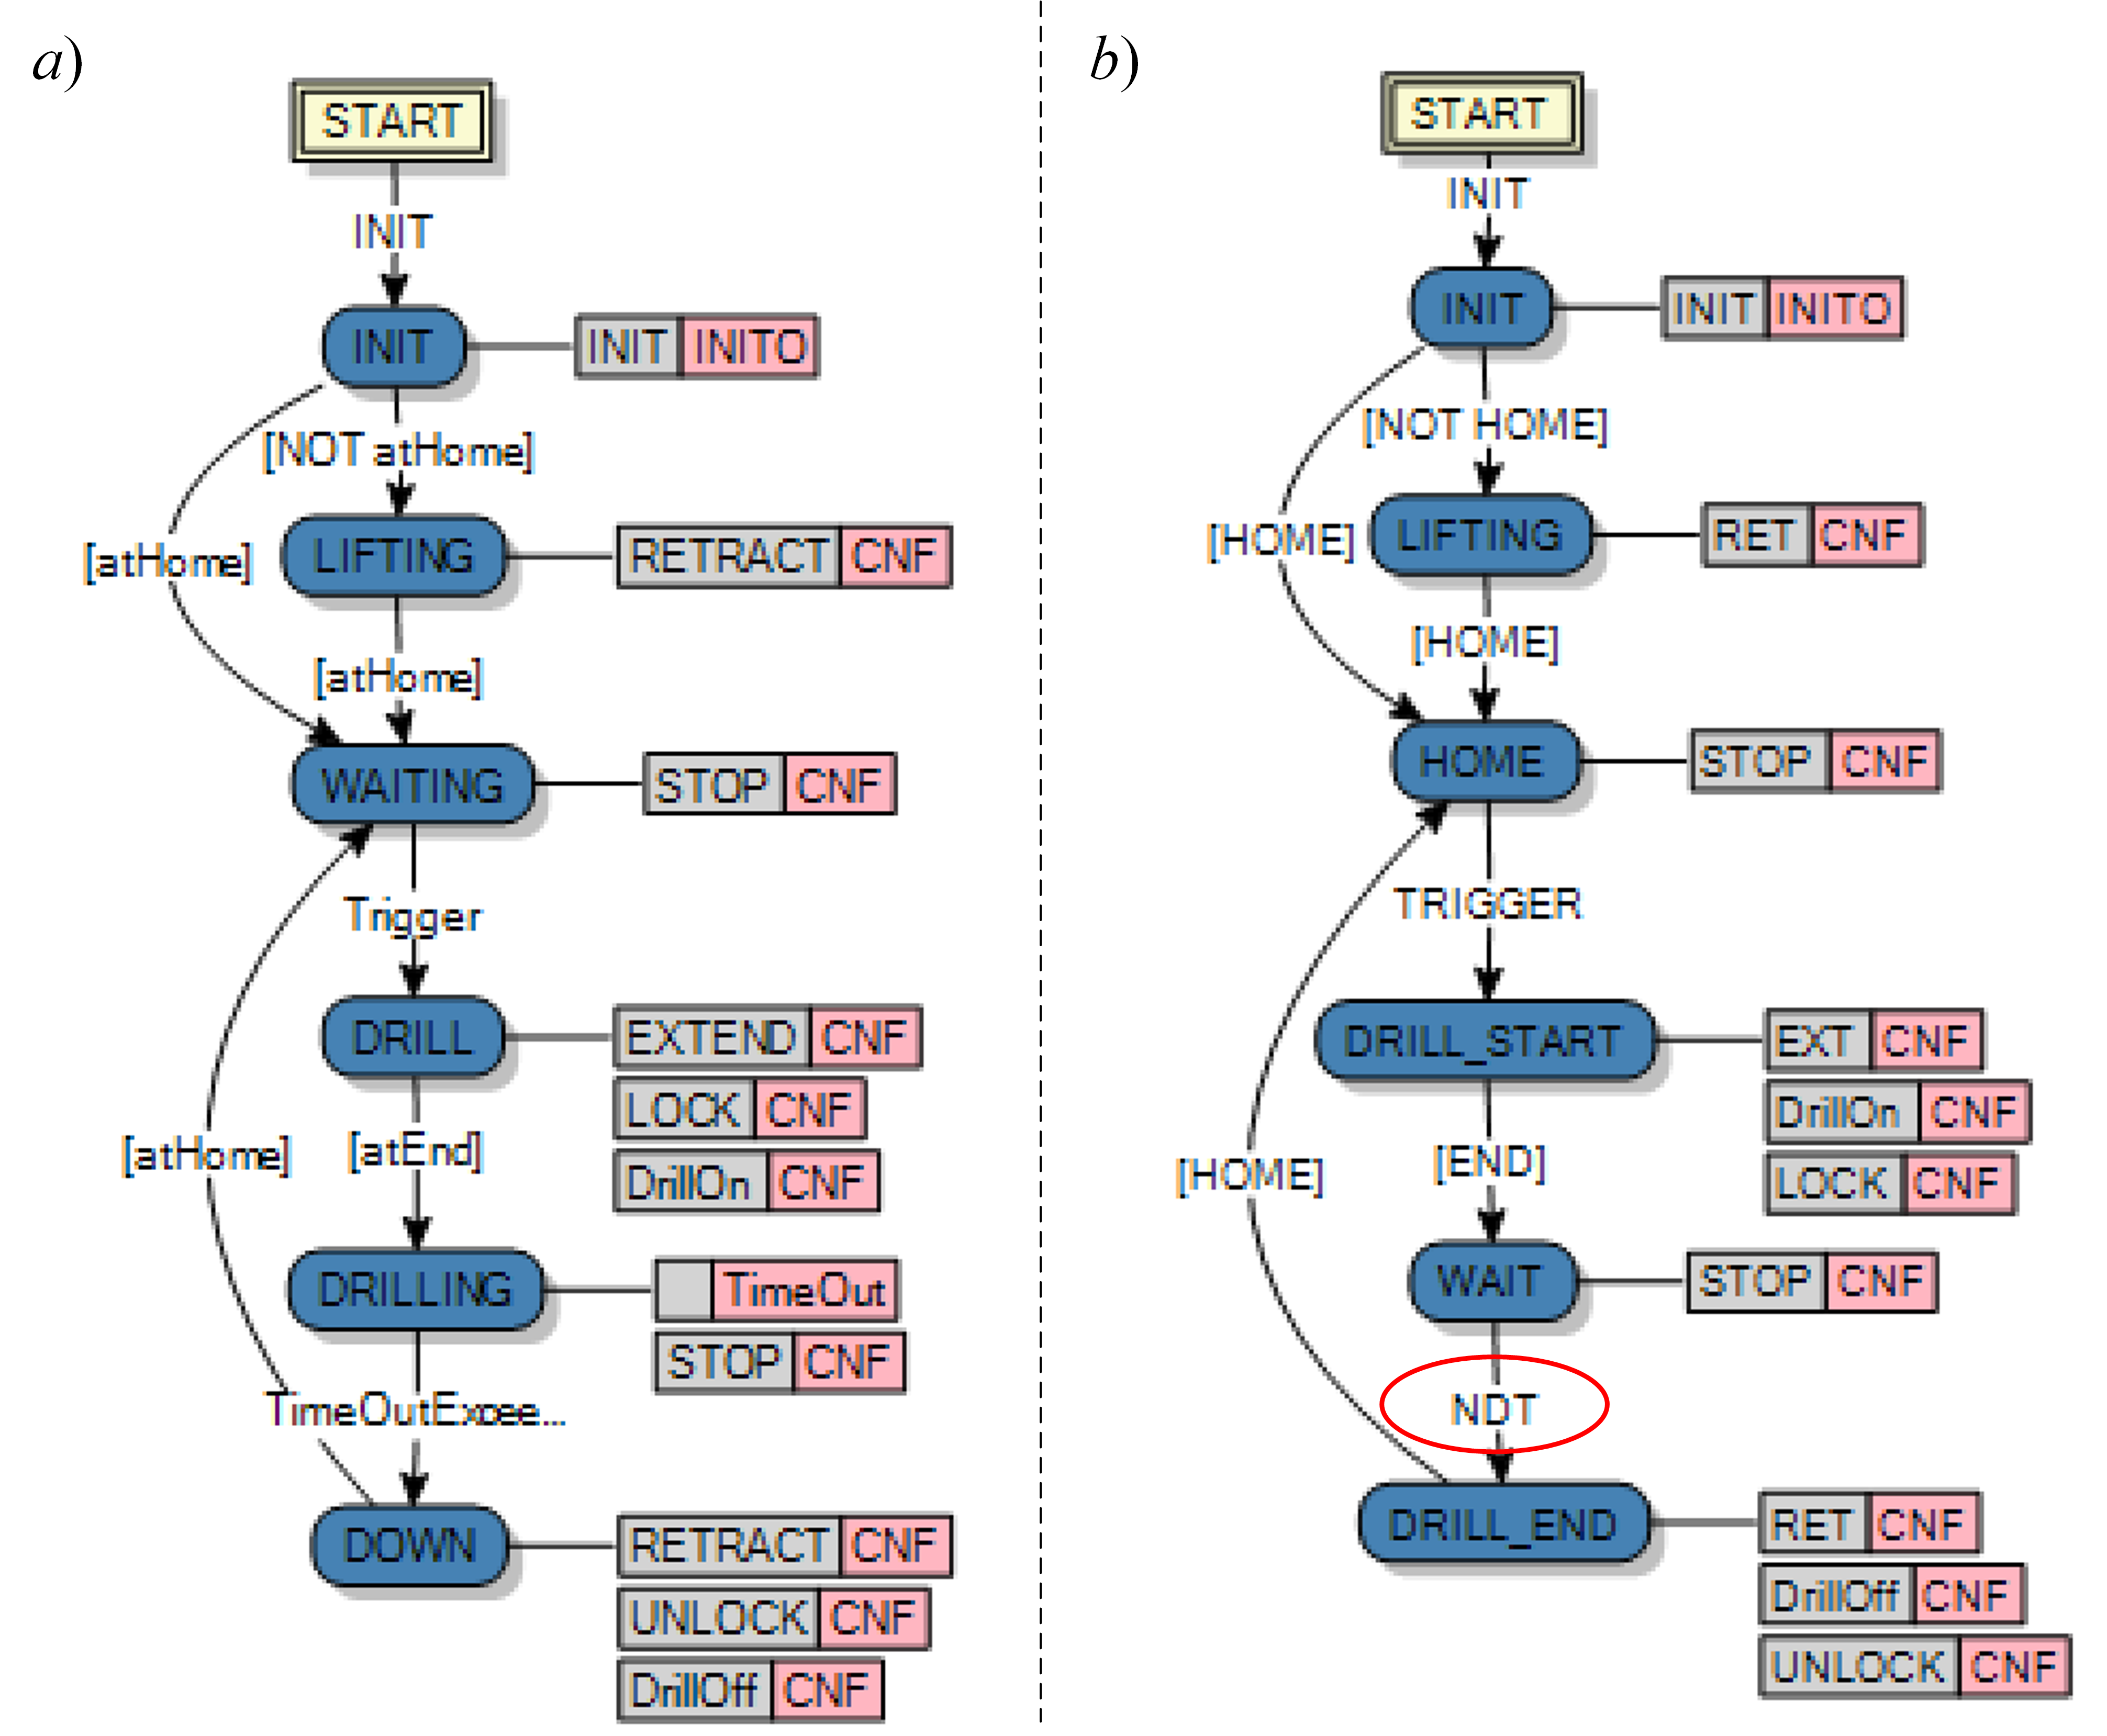
\includegraphics[width=0.8\textwidth]{chapters/images/chapter2/Fig10.png}
\caption{Comparison of controller ECCs: (a) the original drill controller with timer-based delays, and (b) the modified controller using non-deterministic transitions (NDT) for formal verification.}
\label{fig:controller_ndts}
\end{figure}

By connecting the monitor to this ND twin, the model checker can exhaustively test the monitor's logic against all valid controller behaviors. The verification is then guided by two main properties:

\begin{enumerate}
\item The monitor must report a failure when a failure actually occurs. (e.g., G ((m.hext ∧ m.vext) → (m.hext ∧ m.vext U m.collision)))
\item The monitor must not report a spurious failure when the controller is functioning as expected. (e.g., G (¬(m.hext ∧ m.vext) → F ¬m.collision))
\end{enumerate}

This approach ensures that the monitor is trustworthy before it is deployed for online verification, forming a critical link between offline design-time checks and online runtime safety assurance.

\section{Application to Case Studies}\label{sec:case_studies}

The effectiveness of the proposed framework and methodologies has been demonstrated on several case studies, ranging from laboratory-scale systems to real-world safety-critical applications.

\subsection{System of Two Pneumatic Cylinders}

This system involves two orthogonal pneumatic cylinders that must move without colliding. A runtime monitor, NoCollisionMonitor, was implemented as a BFB to ensure this safety property holds during operation. To verify the monitor, an ND twin of the cylinder controller was created. The ND twin was designed to non-deterministically produce EXTEND, RETRACT, and STOP commands, allowing it to generate the collision scenario (EXTEND from both twins simultaneously) as well as all non-collision scenarios. Using NuSMV, the monitor was successfully verified against the two key properties: it correctly reported the collision when it occurred and did not report false positives, proving its reliability.

\subsection{Drilling Station}

This case study features a drilling station with a drill and a rotating table. The control logic, implemented in IEC 61499, was designed to prevent the table from rotating while the drill is active. The system was modeled in a closed loop, with NDTs used in the plant models for the drill and table to represent the unknown duration of their movements. During model checking with NuSMV, a CTL specification G !(DrillCTL\_RET = TRUE \& ActuatorGen\_EO = TRUE) (the table cannot rotate while drilling) was found to be false. The model checker generated a counterexample trace which, after analysis, revealed a flaw in the table controller's ECC that failed to check for a blocking signal before initiating rotation. After fixing the logic and re-running the verification, the property was satisfied, demonstrating the toolchain's ability to find and help correct non-trivial design errors.

\subsection{Safety-Critical Horizontal Handling Machine (HHM)}

The framework was applied to the refactoring and verification of the control software for the HHM, a remote handling robot used to transport highly radioactive material at the SPES nuclear research facility. The original control software, based on IEC 61131, was redesigned using a modular IEC 61499 architecture.

Figure \ref{fig:hhm_control_sequences} presents a critical comparison of two control strategies for the HHM's three linear axes (elevator, trolley, and crane). The left side shows a parallel execution approach where all three axes move simultaneously, which can lead to potential collisions depending on the relative speeds of the movements. The right side demonstrates the safer sequential execution approach, where movements are carefully orchestrated to prevent any possibility of collision. This figure illustrates how the framework can be used to verify that the sequential approach maintains safety properties while the parallel approach may violate them, highlighting the importance of formal verification in safety-critical applications.

\begin{figure}[h]
\centering
\includegraphics[width=0.9\textwidth]{chapters/images/chapter2/lilli09-eps-converted-to.pdf}
\caption{Comparison of control sequences for the HHM: (a) parallel movement of three linear axes, and (b) sequential execution of the three movements. The sequential approach prevents potential collisions between axes.}
\label{fig:hhm_control_sequences}
\end{figure}

A critical safety requirement is to prevent mechanical collisions between the machine's axes. To test this, a design flaw was deliberately introduced into the controller's FSM, changing a sequence of three axis movements from sequential to parallel execution. This type of error is hard to detect via simulation, as a collision may or may not occur depending on the relative speeds of the axes.

The plant models for the linear axes were created with NDTs to model variable movement times. The entire closed-loop system was translated to SMV and verified with NuSMV. The model checker successfully found a violation of the LTL specification designed to prevent collisions. The resulting counterexample trace was imported into FBME for analysis.

The visual trace analysis in FBME made it possible to step through the failure scenario and clearly identify how the parallel execution, under a specific timing sequence explored by NuSMV due to the NDTs, led to the collision. This case study demonstrates the scalability and practical value of the integrated toolchain in ensuring the safety of complex, real-world industrial systems.

Figure \ref{fig:petri_hmi_iec} demonstrates the multi-faceted approach to system modeling and verification that the framework supports. The figure shows how IEC 61499 function blocks can be integrated with both HMI visualization systems and formal Petri net models, creating a comprehensive verification environment. This integration allows engineers to work with familiar graphical tools while simultaneously enabling rigorous formal analysis. The Petri net representation provides a mathematical foundation for verification, while the HMI offers intuitive visualization of system behavior, bridging the gap between formal methods and practical engineering.

\begin{figure}[h]
\centering
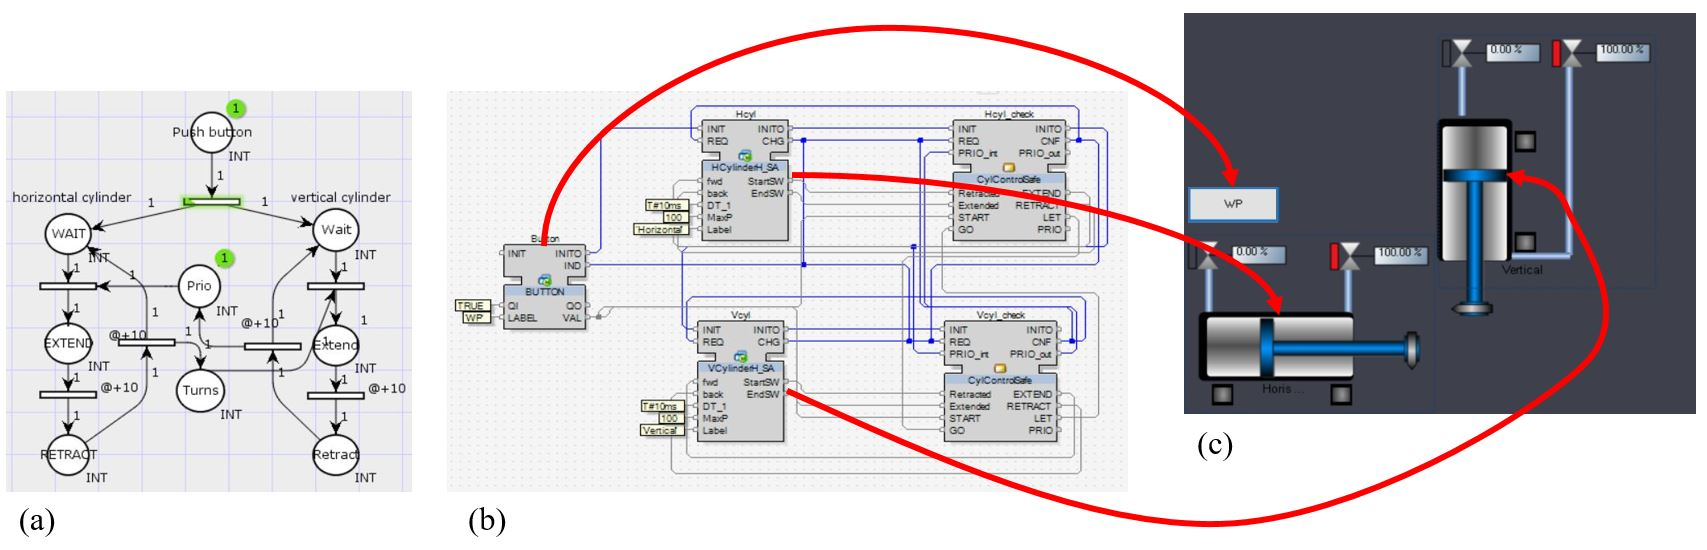
\includegraphics[width=0.7\textwidth]{chapters/images/chapter2/petri_hmi_iec.JPG}
\caption{Integration of IEC 61499 function blocks with HMI visualization and Petri net modeling, showing the relationship between different modeling approaches in the verification framework.}
\label{fig:petri_hmi_iec}
\end{figure}

\section{Conclusion and Future Outlook}\label{sec:conclusion_chapter2}

This chapter presented an integrated framework for the model-based design and formal verification of iCPS developed with the IEC 61499 standard. By combining a seamless toolchain with advanced modeling methodologies, the framework makes the power of formal verification more accessible to automation engineers, enabling the early detection of subtle and critical design flaws that traditional testing methods may miss.

The main contributions are threefold. First, the integrated toolchain provides a practical workflow from design and simulation in standard IDEs to automated formal model generation (fb2smv) , verification (NuSMV) , and intuitive counterexample analysis (FBME). Second, the proposed notation for Non-Deterministic Transitions (NDT) within IEC 61499 plant models allows for the creation of more realistic verification models that can uncover timing-dependent bugs. Third, the methodology for verifying runtime monitors using a non-deterministic twin of the controller ensures that online safety mechanisms are themselves reliable.

The application of this framework to multiple case studies, including a safety-critical nuclear handling system , has validated its effectiveness in improving the dependability of complex distributed automation systems. By lowering the barrier to entry for formal methods, this work contributes to building more robust, reliable, and safer industrial systems.

Future work will focus on extending the framework's capabilities. This includes automating the generation of ND twins for monitor verification and further exploring the scalability of the approach for even larger systems. Another promising direction is the extension of the modeling notation and toolchain to support timed automata, which would allow for the verification of quantitative real-time properties, moving beyond the current focus on logical correctness and untimed non-determinism. Finally, automatically generating specifications from informal requirements and generating plant models from system data logs are active research areas that could further enhance the automation and power of the verification process.
